\label{TasksObserveWeb}
The observation mode for HTML \gdauts{} involves hovering over the component you want to record an action on and pressing a key combination to execute an action on this component:
\begin{itemize}
\item Press  \bxkey{Ctrl+Shift+A} to map that component. 
\item Press \bxkey{Ctrl+Shift+S} to map the application component. 
\end{itemize}

Supported components are marked with red borders (\bxfigref{redborders}). 

\begin{figure}[h]
\begin{center}
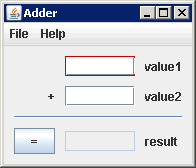
\includegraphics{Tasks/Recording/PS/redborders}
\caption{Red borders in the observation mode}
\label{redborders}
\end{center}
\end{figure}

In the dialog which appears, choose the action you want to execute on this component.

Once you have done this, you can:
\begin{enumerate}
\item Enter the parameters for the action, as prompted by the dialog box.
\bxtipp{You can only enter concrete parameter values in this dialog.}
\item Click \bxcaption{OK} in the dialog.
\item The action you just specified will be carried out.
\item In the \gdtestcaseeditor{} for the \gdcase{} you are observing, the \gdstep{} you just observed will appear. 
\item In the \gdpropview{}, you will see that the \bxname{component} name field contains a name generated by \gd{}. This component name is assigned to the technical name for the component in the \gdomeditor{}. 
\bxtipp{If you change the component name, remember that you will need to reassign your new name to the technical name in the \gdomeditor{}. }
\end{enumerate}

Once you have finished observing your \gdcase{}, stop the observation mode by  
selecting the \bxcaption{stop observing} button on the toolbar. 
 \gdmarpar{../../../share/PS/stopcam}{ stop observation}
\bxtipp{When you are observing, remember that your tests will be more flexible and maintainable if you make the \gdcases{} small, reusable units. }

Save the changes in the editor. 

%checks in the observation mode
